\chapter{Project 1: Threads}

\section{Overview}

The first project strives to improve the current threading system. You are giving a basic threading
system implementation which doesn't account for thread priorities and contains an inefficient timer
implementation. Your job is to improve this functionality by removing the busy waits from the timer
and by making the scheduler take into account thread priorities and solving the problems which arise
from this new scheduler.

Before starting work on the first assignment you should first read and understand
\fullref{chap:Introduction}. You should be able to navigate through the project files in Visual
Studio, compile the code and be able to run the thread tests.

The VS configuration used for compiling the code must be \textbf{Threads}. The only difference
between configuration are the tests which run when building the \textit{RunTests} project.

\subsection{Threading System Initialization}

If you want to understand the whole \projectname load process you can read \fullref{sect:OsStart},
in this section only the flow related to the threading system initialization will be described.

The main thread will be initialized on each CPU in \func{ThreadSystemInitMainForCurrentCPU}. The
initialization sequence for the main thread is shorter compared to creating a new thread, because
its stack already exists and the thread was already 'running' - even if its data structure was
not populated yet.

When this function returns and the main thread is initialized the executive synchronization
mechanisms will be usable: these functions require information about the currently executing thread.

After more system components finish initialization \func{ThreadSystemInitIdleForCurrentCPU} is
called to create the idle thread (this function will also be called on each CPU). After the idle
thread is created the scheduler can now function properly - it has what to schedule in case there
are no threads in the ready list. The function executed by the idle thread can be seen in
\func{\_IdleThread} - it does nothing useful - the only reason it exists is for a consistent view of
the system, i.e. as there must always be a Stark in Winterfell \cite{asoiaf} there must always be a
thread running on each CPU.

After the idle thread is initialized the interrupts will be enabled and every
\macro{SCHEDULER\_TIMER\_INTERRUPT\_TIME\_US} $\mu$s (currently 40ms) a clock interrupt will trigger
on each processor and if the current thread is running on the CPU for more than
\macro{THREAD\_TIME\_SLICE} clock ticks (currently 1) it will yield after it finished handling the
interrupt. This is done in \func{ThreadTick}.

Another reason why a thread may yield the CPU is when it is trying to acquire a resource which is
currently unavailable: this may be a mutex, an executive event or an executive timer.
See \fullref{sect:ExSynch} for implementation details.

Also, executing threads may be nice and give up their CPU time willingly by calling
\func{ThreadYield} anytime.

For creating a new thread you can use the \func{ThreadCreate} function. You can give the thread a
name (useful only for debugging purposes), a priority (currently disregarded), a function from which
to start execution and a pointer to the parameters of the function. The \func{ThreadCreateEx}
version is available for creating threads in the context of a usermode process - you will not need
this function until project 2 when you will work on user-mode threads.

The function specified will start execution with interrupts enabled and you will \textbf{NOT} have
to disable or re-enable interrupts manually. The synchronization mechanisms will do this for short
(executive) or long (primitive) periods of time. See \fullref{sect:Synch} for more details.

The exit point of any thread is \func{ThreadExit} regardless of whether the thread calls it directly,
it finishes the execution of its start function or it is forced terminated by another thread.

We lied to you, the first function executed by newly created kernel threads is not the startup
function you give to \func{ThreadCreate}, actually it's \func{\_ThreadKernelFunction}, see
\fullref{sect:ThreadInit} for the detailed explanation.

If you want to wait for a thread to terminate its execution you can use
\func{ThreadWaitForTermination}, if you want to terminate it forcefully use \func{ThreadTerminate}.
Warning: this is not a good idea and should seldom be used because the thread may be holding some
resources on termination and they will not be freed; as a result other threads may be deadlocked.

If you want more information read \fullref{sect:Threads} and read the code in \file{thread.c}.

\subsection{Synchronization}

\projectname is a multi-threaded OS, i.e. multiple threads may access the same resources
concurrently: this causes race conditions if these critical sections are not protected by
proper synchronization mechanisms.

\projectname is also multi-processor aware and runs on all the CPUs detected in the system. Due to
this fact, you cannot synchronize the code by relying on the \textbf{bad habit} of disabling
interrupts on the current CPU. The thread from the current CPU (the one disabling the interrupts)
will not be interrupted while executing in a critical section, but another thread (on another CPU)
may also access the same data structures concurrently, hence making \textbf{disabling interrupts
useless} for synchronization.

While holding a primitive lock interrupts are disabled until you release it. The only reason why
you'll want to use primitive synchronization mechanisms will be to synchronize code between
interrupt handlers and other functions. Because interrupt handlers can't sleep they cannot wait on
executive resources (mutexes, events or timers). See \fullref{sect:PrimSynch}.

For all the code you'll write you should use executive synchronization mechanisms. The reason why
they are called executive is because the OS manages them. In contrast with the primitive
synchronization mechanisms these do not use busy waiting for resources, these block the current
thread (yielding the CPU) and causing them to become un-schedulable until the resource becomes
available and the thread is signaled.

These mechanisms use primitive locks internally holding them for the least amount of time necessary.
See \func{MutexAcquire} for a good example. The \var{MutexLock} is taken strictly for updating the
mutex data structure. Before returning control to the caller the function restores the original
interruptibility state. See \fullref{sect:ExSynch}.

There should be no busy waiting in your submission. A tight loop that calls \func{ThreadYield} is
one form of busy waiting.

\subsection{Development}

Work together as a \textbf{TEAM}. Think of the design together and piece the code as early as
possible and not on the night before the submission.

Groups that do this often find that two changes conflict with each other, requiring lots of
last-minute debugging. Some groups who have done this have turned in code that did not
even compile or boot, much less pass any tests.

You \textbf{MUST} use a source version control tool such as Git \cite{git} or Hg \cite{tortoiseHg}
(recommended). This way you'll be 'forced' to collaborate and you will be able to easily merge all
your changes in time and see all your teammates code changes.

You will certainly run into many problems, when doing so it is recommended to read the debugging
section (\fullref{chap:Debugging}) for tips and tricks and to validate
each assumption you make (the recommended way is through ASSERTs).
If you're still having problems do not hesitate to contact your TA and ask for help.

\section{Assignment}

In this project your goal is to improve the thread component.
\begin{enumerate}
	\item Improve the timer implementation by removing busy waiting.
	\item Schedule threads according to their priority.
	\item Solve priority inversion problems by implementing priority donation.
\end{enumerate}

\subsection{Timer}

The current implementation for timers uses busy waiting to determine when the timer should trigger.
This is a very \textbf{wasteful} use of system resources: there is NO reason to keep the
CPU busy when other productive threads may be scheduled or - if no thread is ready - to save some
power and conserve your laptop's battery power.

The timer interface is available in \fullref{sect:ExTimer}. A usage example is illustrated in
\fullref{lst:TimerUsage}. For brevity the example does not check the result of \func{ExTimerInit},
however, when you're working on your project we expect you to always check the result of all the
functions you call.

\begin{lstlisting}[caption={Timer Usage Example},label={lst:TimerUsage}]
EX_TIMER timer;

// Initialize a periodic timer to trigger each 2 seconds
ExTimerInit(&timer, ExTimerTypeRelativePeriodic, 2 * SEC_IN_US);

// After the timer is initialized any number of threads may wait for it, however
// until the timer is started, even if the countdown expired, they must not be
// woken up

// Start the timer, if the countdown has already expired all the threads will
// be instantly woken up
ExTimerStart(&timer);

// Wait for the timer to be signaled, blocks the thread until the countdown
// triggers. In the case of one shot timers issuing a wait after the timer
// has expired will cause the calling thread to return immediately. However
// in the case of periodic timers the countdown will restart after all the
// waiting threads have been woken up and threads will be blocked again
// until the countdown triggers again.
ExTimerWait(&timer);

ExTimerWait(&timer);

ExTimerWait(&timer);

// After we have waited for the timer to trigger 3 times we will stop it
// If there are any threads still waiting on the timer they will be all
// woken up when the timer is stopped.
ExTimerStop(&timer);

// Will return instantly if the timer was stopped
ExTimerWait(&timer);

// Uninitialize the timer, free any memory
ExTimerUninit(&timer);
\end{lstlisting}

\subsection{Priority Scheduler}

\projectname  currently implements a basic round-robin scheduler which doesn't take into account
thread priorities when choosing the next thread to run.

Your objective is to prioritize thread execution, the higher priority thread should always be
scheduled before a lower priority one. This means each time a thread is unblocked (resource is now
available) if it has a higher priority than the one running it should be scheduled in place of the
running one.

This statement is true regardless of the resource it waits for: CPU time, mutex, event, timer.

\textbf{NOTE: This must hold true on a system-wide scale and not on a CPU-wide scale, i.e. even if
a higher priority thread unblocks a medium priority thread it may still need to preempt the
execution of a lower priority thread running on a different CPU.}

Thread priorities range from \macro{ThreadPriorityLowest} (0) and \macro{ThreadPriorityMaximum} (31).
Lower numbers correspond to lower priorities, so that priority 0 is the lowest priority and priority
31 the highest. If there’s no reason to choose another priority, use \macro{ThreadPriorityDefault} 
(16). These enums can be found in \file{thread\_defs.h}.

You will have to work with both the scheduling functions (\func{ThreadYield}, 
\func{\_ThreadGetReadyThread}) and with the executive synchronization mechanisms: mutex, events and
timers.

\subsection{Priority Donation}

After we implement the priority scheduler we realize we have a very big problem: \textit{priority
inversion}. Consider high, medium, and low priority threads H, M, and L, respectively. If H needs to 
wait for L (for instance, for a lock held by L), and M is on the ready list, then H will never get 
the CPU because the low priority thread will not get any CPU time. A partial fix for this problem is
for H to “donate” its priority to L while L is holding the lock, then recall the donation once L
releases (and thus H acquires) the lock.

\textbf{NOTE: Even if the L thread may gain the opportunity to run on a multi-core system in
parallel with the M thread we want our OS to run on any compatible system no matter its CPU
configuration. Also, it is logical when a higher priority thread depends on lower priority threads
to boost their priority to be able to unblock the H thread as quickly as possible.}

Implement priority donation. You will need to account for all different situations in which priority 
donation is required. Be sure to handle multiple donations, in which multiple priorities are donated 
to a single thread. You must also handle nested donation: if H is waiting on a lock that M holds and 
M is waiting on a lock that L holds, then both M and L should be boosted to H’s priority. If 
necessary, you may impose a reasonable limit on depth of nested priority donation, such as 8 levels.
See \fullref{fig:PriorityInversion} for an illustration - figure taken from 
\href{http://stackoverflow.com/questions/4252158/what-is-priority-inversion}{Stack Overflow}.

You must implement priority donation for mutexes.

\begin{figure}
	\centering
	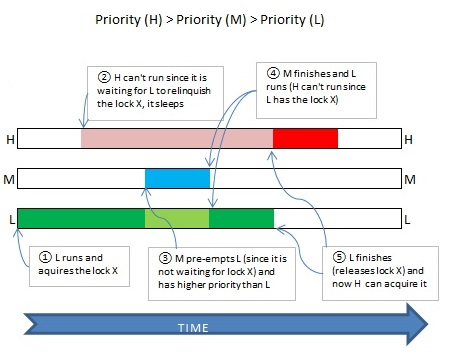
\includegraphics{PriorityInversion}
		\caption{Priority Inversion}
	\label{fig:PriorityInversion}
\end{figure}


\begin{lstlisting}[caption={Thread priority functions},label={lst:PrioFunc}]
//******************************************************************************
// Function:     ThreadGetPriority
// Description:  Returns the thread's priority. In the presence of
//               priority donation, returns the higher(donated) priority.
// Returns:      THREAD_PRIORITY
// Parameter:    IN_OPT PTHREAD Thread - If NULL returns the priority of the
//               current thread.
//******************************************************************************
THREAD_PRIORITY
ThreadGetPriority(
    IN_OPT  PTHREAD             Thread
    );

//******************************************************************************
// Function:     ThreadSetPriority
// Description:  Sets the thread's priority to new priority. If the
//               current thread no longer has the highest priority, yields.
// Returns:      void
// Parameter:    IN THREAD_PRIORITY NewPriority
//******************************************************************************
void
ThreadSetPriority(
    IN      THREAD_PRIORITY     NewPriority
    );
\end{lstlisting}

\subsection{BONUS: Per-CPU ready lists}

\section{Source Files}

We suggest always navigating the project through the Visual Studio interface, because the files are
not organized into folders on the filesystem. In Visual Studio there are filters which group
functionalities. For this project you will work with some of the files in the \textit{executive}
filter.

Here is a quick overview of all the files.

\file{thread.h}

\file{thread\_defs.h}

These are the public thread definitions - these functions may be used by any external components
such as drivers and the syscall interface.

\file{thread\_internal.h}

These functions and structure definitions should only be used by a few components from the OS which
work tightly with the thread functionality. Some examples include the executive synchronization
mechanisms and the interrupt handler which will need access to the \func{ThreadTick},
\func{ThreadBlock}, \func{ThreadYieldOnInterrupt} and other similar functions.

\file{thread.c}

Contains the implementation of the functionality exposed in all the thread* headers. For more
information regarding the functionality and the threading mechanisms see \fullref{sect:Threads}.

\file{\_thread.yasm}

Contains the low-level implementation of the mechanisms required for thread startup and thread
switching. You will NOT have to work in these files, if you are interested in details you can read
\fullref{sect:ThreadSwitch} and \fullref{sect:ThreadInit}.

\file{mutex.h}

\file{mutex.c}

Contains the mutex implementation (a.k.a. executive lock). For more information see 
\fullref{sect:Mutex}. You will have to work here for implementing priority scheduling and donation.

\file{ex\_event.h}

\file{ex\_event.c}

Contains the executive event functionality. For more information see \fullref{sect:ExEvent}. You
don't have to modify these files.

\file{ex\_timer.h}

\file{ex\_timer.c}

Contains the executive timer implementation. You will have to work in the c file to implement the
version without busy waiting. For more information see \fullref{sect:ExTimer}.

\section{FAQ}

\textbf{Q: How much code will I need to write?}

A: Here’s a summary of our reference solution, produced by the hg  diff program. The final row gives
total lines inserted and deleted; a changed line counts as both an insertion and a deletion.

The reference solution represents just one possible solution. Many other solutions are also possible
and many of those differ greatly from the reference solution. Some excellent solutions may not
modify all the files modified by the reference solution, and some may modify files not modified by
the reference solution.

%\begin{figure}
\begin{verbatim}
src/HAL9000/headers/ex_system.h       |   20 +++++
src/HAL9000/headers/ex_timer.h        |   17 +++-
src/HAL9000/headers/mutex.h           |    2 +
src/HAL9000/headers/thread_internal.h |   17 +++++
src/HAL9000/src/ex_event.c            |    4 +-
src/HAL9000/src/ex_system.c           |  247 +++++++++++++++++++++++++++++++++++++++
src/HAL9000/src/ex_timer.c            |   76 ++++++++++++++++-----
src/HAL9000/src/mutex.c               |    7 +-
src/HAL9000/src/system.c              |   10 ++
src/HAL9000/src/thread.c              |  156 +++++++++++++++++++++++++++++++++++++-
src/shared/kernel/thread.h            |    2 +
11 files changed, 525 insertions(+), 33 deletions(-)
\end{verbatim}
%\caption{Threads module changes}
%\label{fig:ThreadsSolution}
%\end{figure} 

\newline

\subsection{Priority Scheduler}

\textbf{Q: Doesn’t priority scheduling lead to starvation?}

A: Yes, strict priority scheduling can lead to starvation because a thread will not run if any 
higher-priority thread is runnable. Strict priority scheduling is valuable in real-time systems 
because it offers the programmer more control over which jobs get processing time. High priorities
are generally reserved for time-critical tasks. It’s not "fair", but it addresses other concerns not
applicable to a general-purpose operating system.

\newline

\textbf{Q: What thread should run after a lock has been released?}

A: When a lock is released, the highest priority thread waiting for that lock should be unblocked 
and put on the list of ready threads. The scheduler should then run the highest priority thread on
the ready list.

\newline

\textbf{Q: If the highest-priority thread yields, does it continue running?}

A: Yes. If there is a single highest-priority thread, it continues running until it blocks or 
finishes, even if it calls \func{ThreadYield}. If multiple threads have the same highest priority,
\func{ThreadYield} should switch among them in round robin order.

\newline

\textbf{Q: Can a thread added to the ready list preempt the processor?}

A: Yes. If a thread added to the ready list has higher priority than the running thread on any
processor, the correct behavior is to immediately schedule the thread on the CPU executing the
lowest priority thread. It is not acceptable to wait for the next timer interrupt. The highest
priority thread should run as soon as it is runnable, preempting whatever thread is currently
running.

\newline

\subsection{Priority Donation}

\textbf{Q: What happens to the priority of a donating thread?}

A: Priority donation only changes the priority of the donee thread. The donor thread’s priority is 
unchanged. Priority donation is not additive: if thread A (with priority 5) donates to thread B 
(with priority 3), then B’s new priority is 5, not 8.

\newline

\textbf{Q: Can a thread’s priority change while it is on the ready queue?}

A: Yes. Consider a ready, low-priority thread L that holds a lock. High-priority thread H attempts 
to acquire the lock and blocks, thereby donating its priority to ready thread L.

\newline

\textbf{Q: Can a thread’s priority change while it is blocked?}

A: Yes. While a thread that has acquired lock L is blocked for any reason, its priority can increase
by priority donation if a higher-priority thread attempts to acquire L.

\newline


\textbf{Q: How does \func{ThreadSetPriority} affect a thread receiving donations?}

A: It sets the thread’s base priority. The thread’s effective priority becomes the higher of the 
newly set priority or the highest donated priority. When the donations are released, the thread’s 
priority becomes the one set through the function call.